\documentclass[a4paper]{article}
\usepackage{fontspec}   %加這個就可以設定字體
\usepackage{xeCJK}       %讓中英文字體分開設置
\usepackage{indentfirst}
\usepackage{listings}
\usepackage[newfloat]{minted}
\usepackage{float}
\usepackage{graphicx}
\usepackage{caption}
\usepackage{fancyhdr}
\usepackage{hyperref}
\usepackage{amsmath}
\usepackage{multirow}
\usepackage[dvipsnames]{xcolor}
\usepackage{graphicx}
\usepackage{tabularx}
\usepackage{booktabs}
\usepackage{caption}
\usepackage{subcaption}
\usepackage{pifont}
\usepackage{amssymb}
\usepackage[backend=biber]{biblatex}
\addbibresource{main.bib}


\usepackage{pdftexcmds}
\usepackage{catchfile}
\usepackage{ifluatex}
\usepackage{ifplatform}

\usepackage[breakable, listings, skins, minted]{tcolorbox}
\usepackage{etoolbox}
\setminted{fontsize=\footnotesize}
\renewtcblisting{minted}{%
    listing engine=minted,
    minted language=python,
    listing only,
    breakable,
    enhanced,
    minted options = {
        linenos, 
        breaklines=true, 
        breakbefore=., 
        % fontsize=\footnotesize, 
        numbersep=2mm
    },
    overlay={%
        \begin{tcbclipinterior}
            \fill[gray!25] (frame.south west) rectangle ([xshift=4mm]frame.north west);
        \end{tcbclipinterior}
    }   
}

\usepackage[
top=1.5cm,
bottom=0.75cm,
left=1.5cm,
right=1.5cm,
includehead,includefoot,
heightrounded, % to avoid spurious underfull messages
]{geometry} 

\newenvironment{code}{\captionsetup{type=listing}}{}
\SetupFloatingEnvironment{listing}{name=Code}



\title{Deep Learning Lab 5 - Value-Based Reinforcement Learning}
\author{110550088 李杰穎}
\date{\today}


\setCJKmainfont{Noto Serif TC}



\ifwindows
\setmonofont[Mapping=tex-text]{Consolas}
\fi

\XeTeXlinebreaklocale "zh"             %這兩行一定要加,中文才能自動換行
\XeTeXlinebreakskip = 0pt plus 1pt     %這兩行一定要加,中文才能自動換行

\newcommand*{\dif}{\mathop{}\!\mathrm{d}}


%\setlength{\parindent}{0em}
%\setlength{\parskip}{2em}
%\renewcommand{\baselinestretch}{1.25}
%\setlength{\droptitle}{-7.5em}   % This is your set screw
%\setlength{\columnsep}{2em}

\begin{document}
\maketitle
\section{Introduction}

In this lab, I implement and enhance the Deep Q-Network (DQN)~\cite{mnih2013playing} algorithm using PyTorch across two distinct environments: the simple CartPole balancing task and the more complex Atari Pong game. The work progresses in strategic stages, beginning with a foundational implementation that successfully achieves maximum scores in both environments through three key components: uniform sampling for experience replay, 1-step returns for value estimation, and $\epsilon$-greedy exploration.

Building on this solid baseline, based on observations in \cite{hessel2018rainbow}, I incorporate advanced DQN enhancements to dramatically improve sample efficiency:

\begin{enumerate}
    \item \textbf{Huber Loss} to increase robustness against outliers and stabilize training
    \item \textbf{Prioritized Experience Replay (PER)} with annealing $\beta$ parameter to focus training on the most informative experiences
    \item \textbf{Double DQN (DDQN)} to reduce overestimation bias in Q-value targets
    \item \textbf{Multi-step Return} to propagate rewards more effectively through time
    \item \textbf{Dueling DQN architecture} to separately estimate state values and action advantages
    \item \textbf{Noisy Networks} for more effective state-dependent exploration
    \item \textbf{Enhanced Frame Preprocessing} to increase the convergence speed of neural networks
\end{enumerate}

The combination of these advanced techniques yields remarkable results: achieving a near-perfect score of 19 in Pong within just 200,000 environment steps, a significant improvement over the standard DQN implementation which typically requires millions of steps to reach comparable performance. This substantial efficiency gain demonstrates the power of integrating multiple algorithmic improvements in deep reinforcement learning.

This report is organized as follows: Section 2 details my implementation of the various DQN components and enhancements. Section 3 presents the experimental results and analysis, including training curves and ablation studies. Finally, Section 4 concludes with key findings and potential future work.

\section{Implementation}
\subsection{Bellman Error for DQN}

The Bellman error for Q-learning represents the difference between the current Q-value estimate and the target Q-value, which is defined as:
\begin{equation}
\delta = r + \gamma \max_{a'} Q(s', a') - Q(s, a),
\end{equation}
where $\delta$ is the Bellman error (also called TD error), $r$ is the current reward, $\gamma$ is the discount factor, $Q(s, a)$ is the Q-value with given state $s$ and action $a$, and $s'$ is the next state.

In DQN, we approximate the Q-value function using a deep neural network. To train this network, we formulate the loss function as the mean squared error of the Bellman error. Formally, the loss function can be written as:
\begin{equation}
L_{DQN}(\theta) := \frac{1}{2} \sum_{(s,a,r,s') \in D} \left( r + \gamma \max_{a' \in A} Q(s', a'; \bar{\theta}) - Q(s, a; \theta) \right)^2,
\end{equation}
where $\theta$ represents the parameters of the main Q-network, $\bar{\theta}$ represents the parameters of the target Q-network, $D$ is the experience replay buffer containing transitions $(s,a,r,s')$, $r$ is the immediate reward, $\gamma$ is the discount factor, $Q(s,a;\theta)$ is the predicted Q-value for state $s$ and action $a$, and $\max_{a' \in A} Q(s',a';\bar{\theta})$ is the maximum Q-value for the next state $s'$ across all possible actions.

The PyTorch implementation of this loss function is:
\begin{code}
\captionof{listing}{\textbf{Implementation of the Bellman loss}}
\label{code:loss}
\begin{minted}
# Get Q-values for current states and actions
q_values = self.q_net(states).gather(1, actions.unsqueeze(1)).squeeze(1)

# Calculate target Q-values using the target network
with torch.no_grad():
    next_q_values = self.target_net(next_states).max(1)[0]
    target_q_values = rewards + (1 - dones) * self.gamma * next_q_values

# Calculate TD errors for updating priorities
td_errors = target_q_values - q_values

# Calculate weighted MSE loss
loss = (weights * (td_errors ** 2)).mean()
\end{minted}
\end{code}

\subsection{Network Architecture}

I implemented two different Q-network architectures: a Multi-Layer Perceptron (MLP) for the CartPole environment and a Convolutional Neural Network (CNN) for the Atari Pong environment. The implementation is flexible and supports various enhancements like dueling architecture and noisy networks:

\begin{code}
\captionof{listing}{\textbf{Implementation of the vanilla DQN}}
\label{code:vanilla_network}
\begin{minted}
class VanillaDQN(nn.Module):
    def __init__(self, input_dim, num_actions, conv=False, hidden_dim=512, dueling=False, noisy=False, vanilla=False):
        super(VanillaDQN, self).__init__()
        self.conv = conv
        self.dueling = dueling
        self.noisy = noisy
        self.num_actions = num_actions
        
        # Choose the appropriate linear layer based on noisy flag
        LinearLayer = NoisyLinear if noisy else nn.Linear
        self.multiplier = 2 if vanilla else 1
        if conv:
            self.network = nn.Sequential(
                nn.Conv2d(input_dim, 16 * self.multiplier, kernel_size=8, stride=4),
                nn.ReLU(),
                nn.Conv2d(16 * self.multiplier, 32 * self.multiplier, kernel_size=4, stride=2),
                nn.ReLU(),
                nn.Conv2d(32 * self.multiplier, 32 * self.multiplier, kernel_size=3, stride=1),
                nn.ReLU(),
                nn.Flatten(),
                LinearLayer(32 * 7 * 7 * self.multiplier, 512),
                nn.ReLU(),
                LinearLayer(512, num_actions)
            )
        else:
            self.network = nn.Sequential(
                LinearLayer(input_dim, hidden_dim),
                nn.ReLU(),
                LinearLayer(hidden_dim, hidden_dim),
                nn.ReLU(),
                LinearLayer(hidden_dim, num_actions)
            )

    def forward(self, x):
        if self.conv:
            x = x / 255.0
            
        return self.network(x)
\end{minted}
\end{code}

\subsection{Huber Loss}

The Huber loss is a robust loss function that combines the benefits of mean squared error (MSE) for small errors and mean absolute error (MAE) for large errors. This makes it less sensitive to outliers than MSE, which is particularly important in RL where rewards and Q-values can sometimes have high variance.

As described in \cite{mnih2015human} in their seminal DQN paper, using the Huber loss instead of MSE can stabilize training by reducing the impact of large TD errors. The Huber loss is defined as:

\begin{equation}
L_{\delta}(y, f(x)) = 
\begin{cases}
\frac{1}{2}(y - f(x))^2 & \text{for } |y - f(x)| \leq \delta \\
\delta (|y - f(x)| - \frac{1}{2}\delta) & \text{otherwise}
\end{cases}
\end{equation}

where $\delta$ is a hyperparameter that determines the threshold between the quadratic and linear regions.

In PyTorch, this is implemented using the \texttt{smooth\_l1\_loss} function:

\begin{code}
\captionof{listing}{\textbf{Implementation of Huber loss}}
\label{code:huber}
\begin{minted}
# Get Q-values for current states and actions
q_values = self.q_net(states).gather(1, actions.unsqueeze(1)).squeeze(1)

# Calculate target Q-values using the target network
with torch.no_grad():
    next_q_values = self.target_net(next_states).max(1)[0]
    target_q_values = rewards + (1 - dones) * self.gamma * next_q_values

# Calculate loss using Huber loss (smooth_l1_loss) with importance sampling weights
loss = (weights * torch.nn.functional.smooth_l1_loss(q_values, target_q_values.detach(), reduction='none')).mean()
\end{minted}
\end{code}

\subsection{Prioritized Experience Replay (PER)}

Prioritized Experience Replay (PER) was introduced by \cite{schaul2016prioritized} to address a key limitation of uniform sampling in experience replay: not all transitions are equally valuable for learning. PER prioritizes transitions with higher TD errors, as these represent experiences from which the agent can learn more.

The key components of PER include:
\begin{itemize}
    \item \textbf{Priority Assignment}: Each transition is assigned a priority proportional to its TD error: $p_i = (|\delta_i| + \epsilon)^\alpha$, where $\epsilon$ is a small positive constant to ensure non-zero sampling probability and $\alpha$ controls the degree of prioritization.
    \item \textbf{Probability Calculation}: The probability of sampling transition $i$ is: $P(i) = \frac{p_i^\alpha}{\sum_k p_k^\alpha}$
    \item \textbf{Importance Sampling}: To correct the bias introduced by prioritized sampling, importance sampling weights are applied to the loss: $w_i = (\frac{1}{N \cdot P(i)})^\beta$, where $\beta$ is annealed from its initial value to 1 over the course of training.
\end{itemize}

My implementation features a gradual increase of $\beta$ to ensure proper bias correction as training progresses:

\begin{code}
\captionof{listing}{\textbf{Implementation of Prioritized Experience Replay}}
\label{code:per}
\begin{minted}
class PrioritizedReplayBuffer:
    """
        Prioritizing the samples in the replay memory by the Bellman error
        See the paper (Schaul et al., 2016) at https://arxiv.org/abs/1511.05952
    """ 
    def __init__(self, capacity, alpha=0.7, beta=0.4):
        self.capacity = capacity
        self.alpha = alpha
        self.beta = beta
        self.beta_increment = (1.0 - beta) / 200_000  # Increment beta gradually
        self.buffer = []
        self.priorities = np.zeros((capacity,), dtype=np.float32)
        self.max_priority = 1.0
        self.pos = 0

    def add(self, transition, error=None):
        # Calculate priority based on TD error
        if error is None:
            priority = self.max_priority
        else:
            priority = (abs(error) + 1e-5) ** self.alpha
        
        # Add transition to buffer
        if len(self.buffer) < self.capacity:
            self.buffer.append(transition)
        else:
            self.buffer[self.pos] = transition
        
        # Update priority
        self.priorities[self.pos] = priority
        self.pos = (self.pos + 1) % self.capacity
        
    def sample(self, batch_size):
        # If buffer is empty or not enough samples, return None
        if len(self.buffer) == 0:
            return None, None, None, None, None, None
        if len(self.buffer) < batch_size:
            batch_size = len(self.buffer)
        
        # Calculate sampling probabilities
        priorities = self.priorities[:len(self.buffer)]
        probabilities = priorities / np.sum(priorities)
        
        # Sample indices based on the probabilities
        indices = np.random.choice(len(self.buffer), batch_size, p=probabilities, replace=False)
        
        # Calculate importance sampling weights
        weights = (len(self.buffer) * probabilities[indices]) ** (-self.beta)
        weights /= weights.max()  # Normalize weights
        
        # Gradually increase beta to 1
        self.beta = min(1.0, self.beta + self.beta_increment)
        
        # Get the sampled transitions
        batch = [self.buffer[i] for i in indices]
        states, actions, rewards, next_states, dones = zip(*batch)
        
        return states, actions, rewards, next_states, dones, indices, weights
    
    def update_priorities(self, indices, errors):
        # Update the priorities of the sampled transitions
        for idx, error in zip(indices, errors):
            # Ensure idx is within valid range
            if idx < len(self.buffer):
                # Calculate new priority and update
                self.priorities[idx] = (abs(error) + 1e-5) ** self.alpha
                self.max_priority = max(self.max_priority, self.priorities[idx])
        return
\end{minted}
\end{code}

\subsection{Double DQN}

Double DQN (DDQN) was proposed by \cite{van2016deep} to address the overestimation bias present in standard DQN. In vanilla DQN, both action selection and value estimation for the next state use the same target network, which can lead to overestimation of Q-values.

DDQN decouples action selection and value estimation by:
1. Using the online network to select the best action for the next state
2. Using the target network to evaluate the Q-value of that action

The DDQN loss function is expressed as:
\begin{equation}
L_{DDQN}(\theta) := frac{1}{2} \sum_{(s,a,r,s') \in D} \left( r + \gamma Q(s', \arg\max_{a' \in A} Q(s', a'; \theta); \bar{\theta}) - Q(s, a; \theta) \right)^2
\end{equation}

Here's my implementation of DDQN:

\begin{code}
\captionof{listing}{\textbf{Implementation of the double DQN (DDQN)}}
\label{code:ddqn}
\begin{minted}
# Get Q-values for current states and actions
q_values = self.q_net(states).gather(1, actions.unsqueeze(1)).squeeze(1)

with torch.no_grad():
    # DDQN: Use online network to select actions, target network to evaluate
    next_actions = self.q_net(next_states).argmax(1, keepdim=True)
    next_q_values = self.target_net(next_states).gather(1, next_actions).squeeze(1)
    
    # Calculate target Q-values
    target_q_values = rewards + (1 - dones) * self.gamma * next_q_values

# Calculate loss using Huber loss with importance sampling weights
loss = (weights * torch.nn.functional.smooth_l1_loss(q_values, target_q_values.detach(), reduction='none')).mean()
\end{minted}
\end{code}

\subsection{Multi-step Return}

Multi-step returns, as described in Sutton and Barto's Reinforcement Learning textbook~\cite{sutton2018reinforcement}, allow the agent to learn from longer reward sequences. Instead of just considering the immediate reward and the estimated value of the next state (1-step return), multi-step returns accumulate rewards over several time steps before bootstrapping with the estimated value.

The n-step return is defined as:
\begin{equation}
R^{(n)}_t = \sum_{k=0}^{n-1} \gamma^k r_{t+k} + \gamma^n \max_{a'} Q(s_{t+n}, a')
\end{equation}

This approach provides a balance between bias and variance in the return estimates. A larger n reduces bias by incorporating more actual rewards, but can increase variance if the environment is stochastic.

In my implementation, I use a fixed-size deque as a buffer to store the last $n$ transitions. For each new transition, I calculate the n-step return using the stored transitions and add it to the replay buffer:

\begin{code}
\captionof{listing}{\textbf{Implementation of multi-step return}}
\label{code:msr}
\begin{minted}
# Main training loop
while not done and step_count < self.max_episode_steps:
    action = self.select_action(state)
    next_obs, reward, terminated, truncated, _ = self.env.step(action)
    done = terminated or truncated
    
    next_state = self.preprocessor.step(next_obs)
    
    # Add to n-step buffer
    self.n_step_buffer.append((state, action, reward, next_state, done))
    
    if len(self.n_step_buffer) == self.n_step:
        # Get initial state and action
        init_state, init_action, _, _, _ = self.n_step_buffer[0]
        
        # Calculate n-step return: sum of discounted rewards
        n_step_return = sum([r * (self.gamma ** i) for i, (_, _, r, _, _) in enumerate(self.n_step_buffer)])
        
        # Get final next state and done flag
        final_next_state = self.n_step_buffer[-1][3]
        final_done = self.n_step_buffer[-1][4]
        
        # Add to replay buffer with n-step information
        self.memory.add((init_state, init_action, n_step_return, final_next_state, final_done), error=None)
    
    elif self.n_step == 1:  # Fallback to 1-step return if n_step is set to 1
        self.memory.add((state, action, reward, next_state, done), error=None)
\end{minted}
\end{code}
\subsection{Dueling Network}

The Dueling Network architecture, introduced by \cite{wang2016dueling}, represents a significant advancement in DQN design by decomposing the Q-function into two separate components: a state value function $V(s)$ and an advantage function $A(s,a)$. This decomposition allows the network to learn which states are valuable independently from learning the effect of each action.

Mathematically, the standard Q-function can be expressed as:

\begin{equation}
Q(s,a) = V(s) + A(s,a)
\end{equation}

Where $V(s)$ represents the intrinsic value of being in state $s$ regardless of the action taken, and $A(s,a)$ represents the relative advantage of taking action $a$ in state $s$ compared to other actions.

However, this decomposition creates an identifiability issue because adding a constant to $V(s)$ and subtracting the same constant from $A(s,a)$ results in the same Q-value. To address this, the dueling architecture forces the advantage function to have zero mean across all actions:

\begin{equation}
Q(s,a) = V(s) + \left(A(s,a) - \frac{1}{|A|}\sum_{a'}A(s,a')\right)
\end{equation}

In my implementation, I created separate value and advantage streams after the shared feature extraction layers:

\begin{code}
\captionof{listing}{\textbf{Implementation of the Dueling Network}}
\label{code:dueling}
\begin{minted}
class DQN(nn.Module):
    """
    DQN with optional dueling architecture and noisy networks
    """
    def __init__(self, input_dim, num_actions, conv=False, hidden_dim=64, dueling=False, noisy=False):
        super(DQN, self).__init__()
        self.conv = conv
        self.dueling = dueling
        self.noisy = noisy
        self.num_actions = num_actions
        
        # Choose the appropriate linear layer based on noisy flag
        LinearLayer = NoisyLinear if noisy else nn.Linear
        
        if conv:
            # Feature extraction layers for convolutional input
            self.features = nn.Sequential(
                nn.Conv2d(input_dim, 16, kernel_size=8, stride=4),
                nn.ReLU(),
                nn.Conv2d(16, 32, kernel_size=4, stride=2),
                nn.ReLU(),
                nn.Conv2d(32, 32, kernel_size=3, stride=1),
                nn.ReLU(),
                nn.Flatten()
            )
            
            feature_output_dim = 32 * 7 * 7
            self.value_stream = nn.Sequential(
                LinearLayer(feature_output_dim, 256),
                nn.ReLU(),
                LinearLayer(256, 1)
            )
            
            self.advantage_stream = nn.Sequential(
                LinearLayer(feature_output_dim, 256),
                nn.ReLU(),
                LinearLayer(256, num_actions)
            )
    def forward(self, x):
        if self.conv:
            x = x / 255.0
            
        features = self.features(x)
        values = self.value_stream(features)
        advantages = self.advantage_stream(features)
        
        # Combine value and advantage streams using the dueling formula
        # Q(s,a) = V(s) + (A(s,a) - mean(A(s,:)))
        return values + (advantages - advantages.mean(dim=1, keepdim=True))
\end{minted}
\end{code}

The dueling architecture offers several key benefits that improved my DQN implementation:

\begin{enumerate}
\item \textbf{Improved state value estimation}: The dedicated value stream can learn the value of being in specific states without considering all possible actions, which is particularly important in Pong where recognizing advantageous ball positions is critical.
\item \textbf{More efficient action selection}: The advantage stream focuses exclusively on determining which actions are better than others in a given state, rather than trying to learn absolute Q-values for each action.
\item \textbf{Reduced overestimation bias}: By separating value and advantage estimation, the architecture helps mitigate the overestimation bias that often affects standard DQN, complementing the effect of Double DQN.
\item \textbf{Better generalization}: The value stream generalizes across actions, providing better estimates for states even when certain actions are rarely taken during training.
\end{enumerate}

\subsection{Noisy Networks}

Noisy Networks, introduced by \cite{fortunato2018noisy}, offer a more sophisticated exploration strategy compared to $\epsilon$-greedy. Instead of randomly selecting actions with a fixed probability, Noisy Networks inject parameterized noise directly into the network weights, allowing for state-dependent exploration.

The key advantages of Noisy Networks include:
\begin{enumerate}
\item State-dependent exploration that adapts to the agent's uncertainty
\item No need for manually decreasing exploration rates
\item More directed exploration compared to random $\epsilon$-greedy actions
\end{enumerate} 

In my implementation, I replace standard linear layers with noisy linear layers that add parameterized noise to weights and biases during forward passes:

\begin{code}
\captionof{listing}{\textbf{Implementation of the Noisy linear layer}}
\label{code:noisy}
\begin{minted}
class NoisyLinear(nn.Module):
    """
    Noisy Linear Layer for exploration
    Based on the paper: Noisy Networks for Exploration (Fortunato et al., 2018)
    """
    def __init__(self, in_features, out_features, sigma_init=0.5):
        super(NoisyLinear, self).__init__()
        self.in_features = in_features
        self.out_features = out_features
        self.sigma_init = sigma_init
        
        # Learnable parameters
        self.weight_mu = nn.Parameter(torch.Tensor(out_features, in_features))
        self.weight_sigma = nn.Parameter(torch.Tensor(out_features, in_features))
        self.bias_mu = nn.Parameter(torch.Tensor(out_features))
        self.bias_sigma = nn.Parameter(torch.Tensor(out_features))
        
        # Register buffers for noise
        self.register_buffer('weight_epsilon', torch.Tensor(out_features, in_features))
        self.register_buffer('bias_epsilon', torch.Tensor(out_features))
        
        # Initialize parameters
        self.reset_parameters()
        self.reset_noise()
    
    def reset_parameters(self):
        mu_range = 1 / np.sqrt(self.in_features)
        self.weight_mu.data.uniform_(-mu_range, mu_range)
        self.weight_sigma.data.fill_(self.sigma_init / np.sqrt(self.in_features))
        self.bias_mu.data.uniform_(-mu_range, mu_range)
        self.bias_sigma.data.fill_(self.sigma_init / np.sqrt(self.out_features))
    
    def reset_noise(self):
        epsilon_in = self._scale_noise(self.in_features)
        epsilon_out = self._scale_noise(self.out_features)
        
        # Factorized Gaussian noise (outer product)
        self.weight_epsilon.copy_(torch.outer(epsilon_out, epsilon_in))
        self.bias_epsilon.copy_(epsilon_out)
    
    def _scale_noise(self, size):
        # Generate Gaussian noise and apply scaling transformation f(x) = sgn(x) * sqrt(|x|)
        x = torch.randn(size)
        return x.sign().mul_(x.abs().sqrt_())
    
    def forward(self, x):
        if self.training:
            # During training, use noisy weights
            weight = self.weight_mu + self.weight_sigma * self.weight_epsilon
            bias = self.bias_mu + self.bias_sigma * self.bias_epsilon
        else:
            # During evaluation, use just the expected weights
            weight = self.weight_mu
            bias = self.bias_mu
        
        return F.linear(x, weight, bias)
\end{minted}
\end{code}

\subsection{Enhanced Frame Preprocessing}

Effective preprocessing of visual inputs is crucial for DQN performance in Atari environments. I implemented several key optimizations beyond standard techniques to significantly improve both learning efficiency and final performance. My preprocessing pipeline includes:

\begin{enumerate}
    \item \textbf{Selective region cropping}: I removed the score area and other irrelevant regions (rows 34-194) from the original 210×160 frames. This focused the network's attention on the gameplay area while reducing input dimensionality by approximately 25\%.
    
    \item \textbf{Binary thresholding}: After grayscale conversion and resizing, I applied binary thresholding with a threshold value of 127. This transformation creates high-contrast frames where the paddles and ball are clearly distinguished from the background. For Pong specifically, this simplification allows the CNN to more easily identify critical game elements without being distracted by unnecessary gradient information.
    
    \item \textbf{Frame stacking}: To capture temporal dynamics (particularly critical for determining ball direction and speed), I maintained a history of 4 consecutive frames. This standard technique from the original DQN paper provides the network with motion information despite using static convolutional layers.
\end{enumerate}

These preprocessing steps collectively transform the raw 210×160×3 RGB input into a more efficient 84×84×4 representation of binary frames. The binary thresholding proved particularly effective for Pong, where the high-contrast representation made it easier for the network to track the small, fast-moving balls.

\begin{code}
\captionof{listing}{\textbf{Implementation of Enhanced Frame Preprocessing}}
\label{code:preprocessing}
\begin{minted}
class AtariPreprocessor:
    """
    Preprocessing the state input of DQN for Atari
    """    
    def __init__(self, frame_stack=4):
        self.frame_stack = frame_stack
        self.frames = deque(maxlen=frame_stack)

    def preprocess(self, obs):
        # Convert to grayscale
        gray = cv2.cvtColor(obs, cv2.COLOR_RGB2GRAY)
        
        # Crop irrelevant parts
        gray = gray[34:194, :]
        
        # Resize to 84x84
        resized = cv2.resize(gray, (84, 84), interpolation=cv2.INTER_AREA)
        _, thresholded = cv2.threshold(resized, 127, 255, cv2.THRESH_BINARY)
        
        return thresholded

    def reset(self, obs):
        frame = self.preprocess(obs)
        self.frames = deque([frame for _ in range(self.frame_stack)], maxlen=self.frame_stack)
        return np.stack(self.frames, axis=0)

    def step(self, obs):
        frame = self.preprocess(obs)
        self.frames.append(frame)
        return np.stack(self.frames, axis=0)
\end{minted}
\end{code}


\subsection{Weights \& Biases Integration}

To systematically track the performance of our various DQN implementations, I employed Weights \& Biases (wandb), a powerful experiment tracking tool. This integration allowed for real-time visualization of training progress, comparison between different algorithmic variants, and efficient hyperparameter tracking.

The implementation consists of three main components:

\begin{code}
\captionof{listing}{\textbf{Implementation of Weights \& Biases initialization}}
\label{code:wandb_init}
\begin{minted}
wandb.init(
    project="DLP-Lab5-DQN-CartPole", 
    name=args.wandb_run_name, 
    save_code=True,
    config=vars(args)
)
\end{minted}
\end{code}

For tracking training progress, I implemented structured logging at different timescales to capture both immediate feedback and long-term trends:

\begin{code}
\captionof{listing}{\textbf{Periodic metric logging during training}}
\label{code:wandb_training}
\begin{minted}
if self.env_count % 1000 == 0:                 
    print(f"[Collect] Ep: {ep} Step: {step_count} SC: {self.env_count} UC: {self.train_count} Eps: {self.epsilon:.4f}")
    wandb.log({
        "Episode": ep,
        "Step Count": step_count,
        "Env Step Count": self.env_count,
        "Update Count": self.train_count,
        "Epsilon": self.epsilon
    })
    # Additional wandb logs for debugging
    wandb.log({
        "Memory Size": len(self.memory),
        "Beta": self.memory.beta
    })

if self.train_count % 1000 == 0:
    print(f"[Train #{self.train_count}] Loss: {loss.item():.4f} Q mean: {q_values.mean().item():.3f} std: {q_values.std().item():.3f}")
    wandb.log({
        "Training Loss": loss.item(),
        "Q Values Mean": q_values.mean().item(),
        "Q Values Std": q_values.std().item(),
        "Target Q Values Mean": target_q_values.mean().item()
    })
\end{minted}
\end{code}

For evaluation and milestone tracking, I implemented as follow:

\begin{code}
\captionof{listing}{\textbf{Evaluation and milestone logging}}
\label{code:wandb_eval}
\begin{minted}
# Check for milestone steps
for milestone in self.milestone_steps:
    if self.env_count >= milestone and milestone not in self.saved_milestones:
        model_path = os.path.join(self.save_dir, f"model_step{milestone}.pt")
        torch.save(self.q_net.state_dict(), model_path)
        print(f"[Milestone] Saved checkpoint at {milestone} environment steps to {model_path}")
        wandb.log({
            "Milestone": milestone,
            "Checkpoint Saved": True
        })
        self.saved_milestones.add(milestone)
        
        # Evaluate at milestone
        eval_rewards = []
        for _ in range(10):
            eval_reward = self.evaluate()
            eval_rewards.append(eval_reward)
        avg_eval_reward = sum(eval_rewards) / len(eval_rewards)
        print(f"[Milestone Eval] Step: {milestone} Avg Eval Reward: {avg_eval_reward:.2f}")
        wandb.log({
            "Milestone": milestone,
            "Milestone Eval Reward": avg_eval_reward
        })
\end{minted}
\end{code}

In the end of episode, I also evaluate the agent performance, and logged as follow:
\begin{code}
\captionof{listing}{\textbf{Implementation of end-of-episode logging}}
\label{code:end}
\begin{minted}
wandb.log({
    "Episode": ep,
    "Total Reward": total_reward,
    "Env Step Count": self.env_count,
    "Update Count": self.train_count,
    "Epsilon": self.epsilon,
})
# Additional end-of-episode logging
wandb.log({
    "Episode Length": step_count,
    "Average Reward": total_reward / max(1, step_count)
})
if ep % 20 == 0:
    eval_rewards = []
    for _ in range(10):
        eval_reward = self.evaluate()
        eval_rewards.append(eval_reward)
    avg_eval_reward = sum(eval_rewards) / len(eval_rewards)
    if avg_eval_reward > self.best_reward:
        self.best_reward = avg_eval_reward
        model_path = os.path.join(self.save_dir, "best_model.pt")
        torch.save(self.q_net.state_dict(), model_path)
        print(f"Saved new best model to {model_path} with reward {avg_eval_reward}")
    print(f"[TrueEval] Ep: {ep} Avg Eval Reward: {avg_eval_reward:.2f} SC: {self.env_count} UC: {self.train_count}")
    wandb.log({
        "Env Step Count": self.env_count,
        "Update Count": self.train_count,
        "Eval Reward": avg_eval_reward
    })
\end{minted}
\end{code}

\section{Analysis and Discussions}

\subsection{Hyperparameters}

The selection of appropriate hyperparameters is critical for DQN performance. Following Rainbow~\cite{hessel2018rainbow}, I used Adam optimizer with learning rate of $0.0001$ and $\epsilon=1.5\text{e-}4$ to ensure stable optimization. My complete hyperparameter configuration for the enhanced DQN is detailed below:

\begin{table}[H]
\centering
\caption{Hyperparameter settings for the enhanced DQN implementation}
\label{tab:hyperparams}
\begin{tabular}{ll}
\toprule
\textbf{Hyperparameter} & \textbf{Value} \\
\midrule
\multicolumn{2}{l}{\textit{Optimization}} \\
Learning rate & $1\text{e-}4$ \\
Optimizer & Adam ($\epsilon=1.5\text{e-}4$) \\
Batch size & 32 \\
Discount factor ($\gamma$) & 0.99 \\
\midrule
\multicolumn{2}{l}{\textit{Network Architecture}} \\
Double DQN & Enabled \\
Dueling architecture & Enabled \\
Noisy networks & Enabled \\
\midrule
\multicolumn{2}{l}{\textit{Replay Buffer}} \\
Memory size & 50,000 transitions \\
Replay buffer type & Prioritized (PER) \\
PER $\alpha$ & 0.7 \\
PER initial $\beta$ & 0.4 \\
n-step returns & 3 \\
\midrule
\multicolumn{2}{l}{\textit{Training Strategy}} \\
Target network update frequency & Every 500 training steps \\
Replay start size & 5,000 transitions \\
Maximum episode steps & 100,000 steps \\
Training frequency & Every 4 environment steps \\
Updates per training cycle & 4 updates \\
\bottomrule
\end{tabular}
\end{table}

These hyperparameters were selected through grid search, with particular attention to the interaction between n-step returns, update frequency, and prioritized replay parameters, as these components significantly impact sample efficiency.


\subsection{Training Curves}


\begin{figure}[H]
\centering
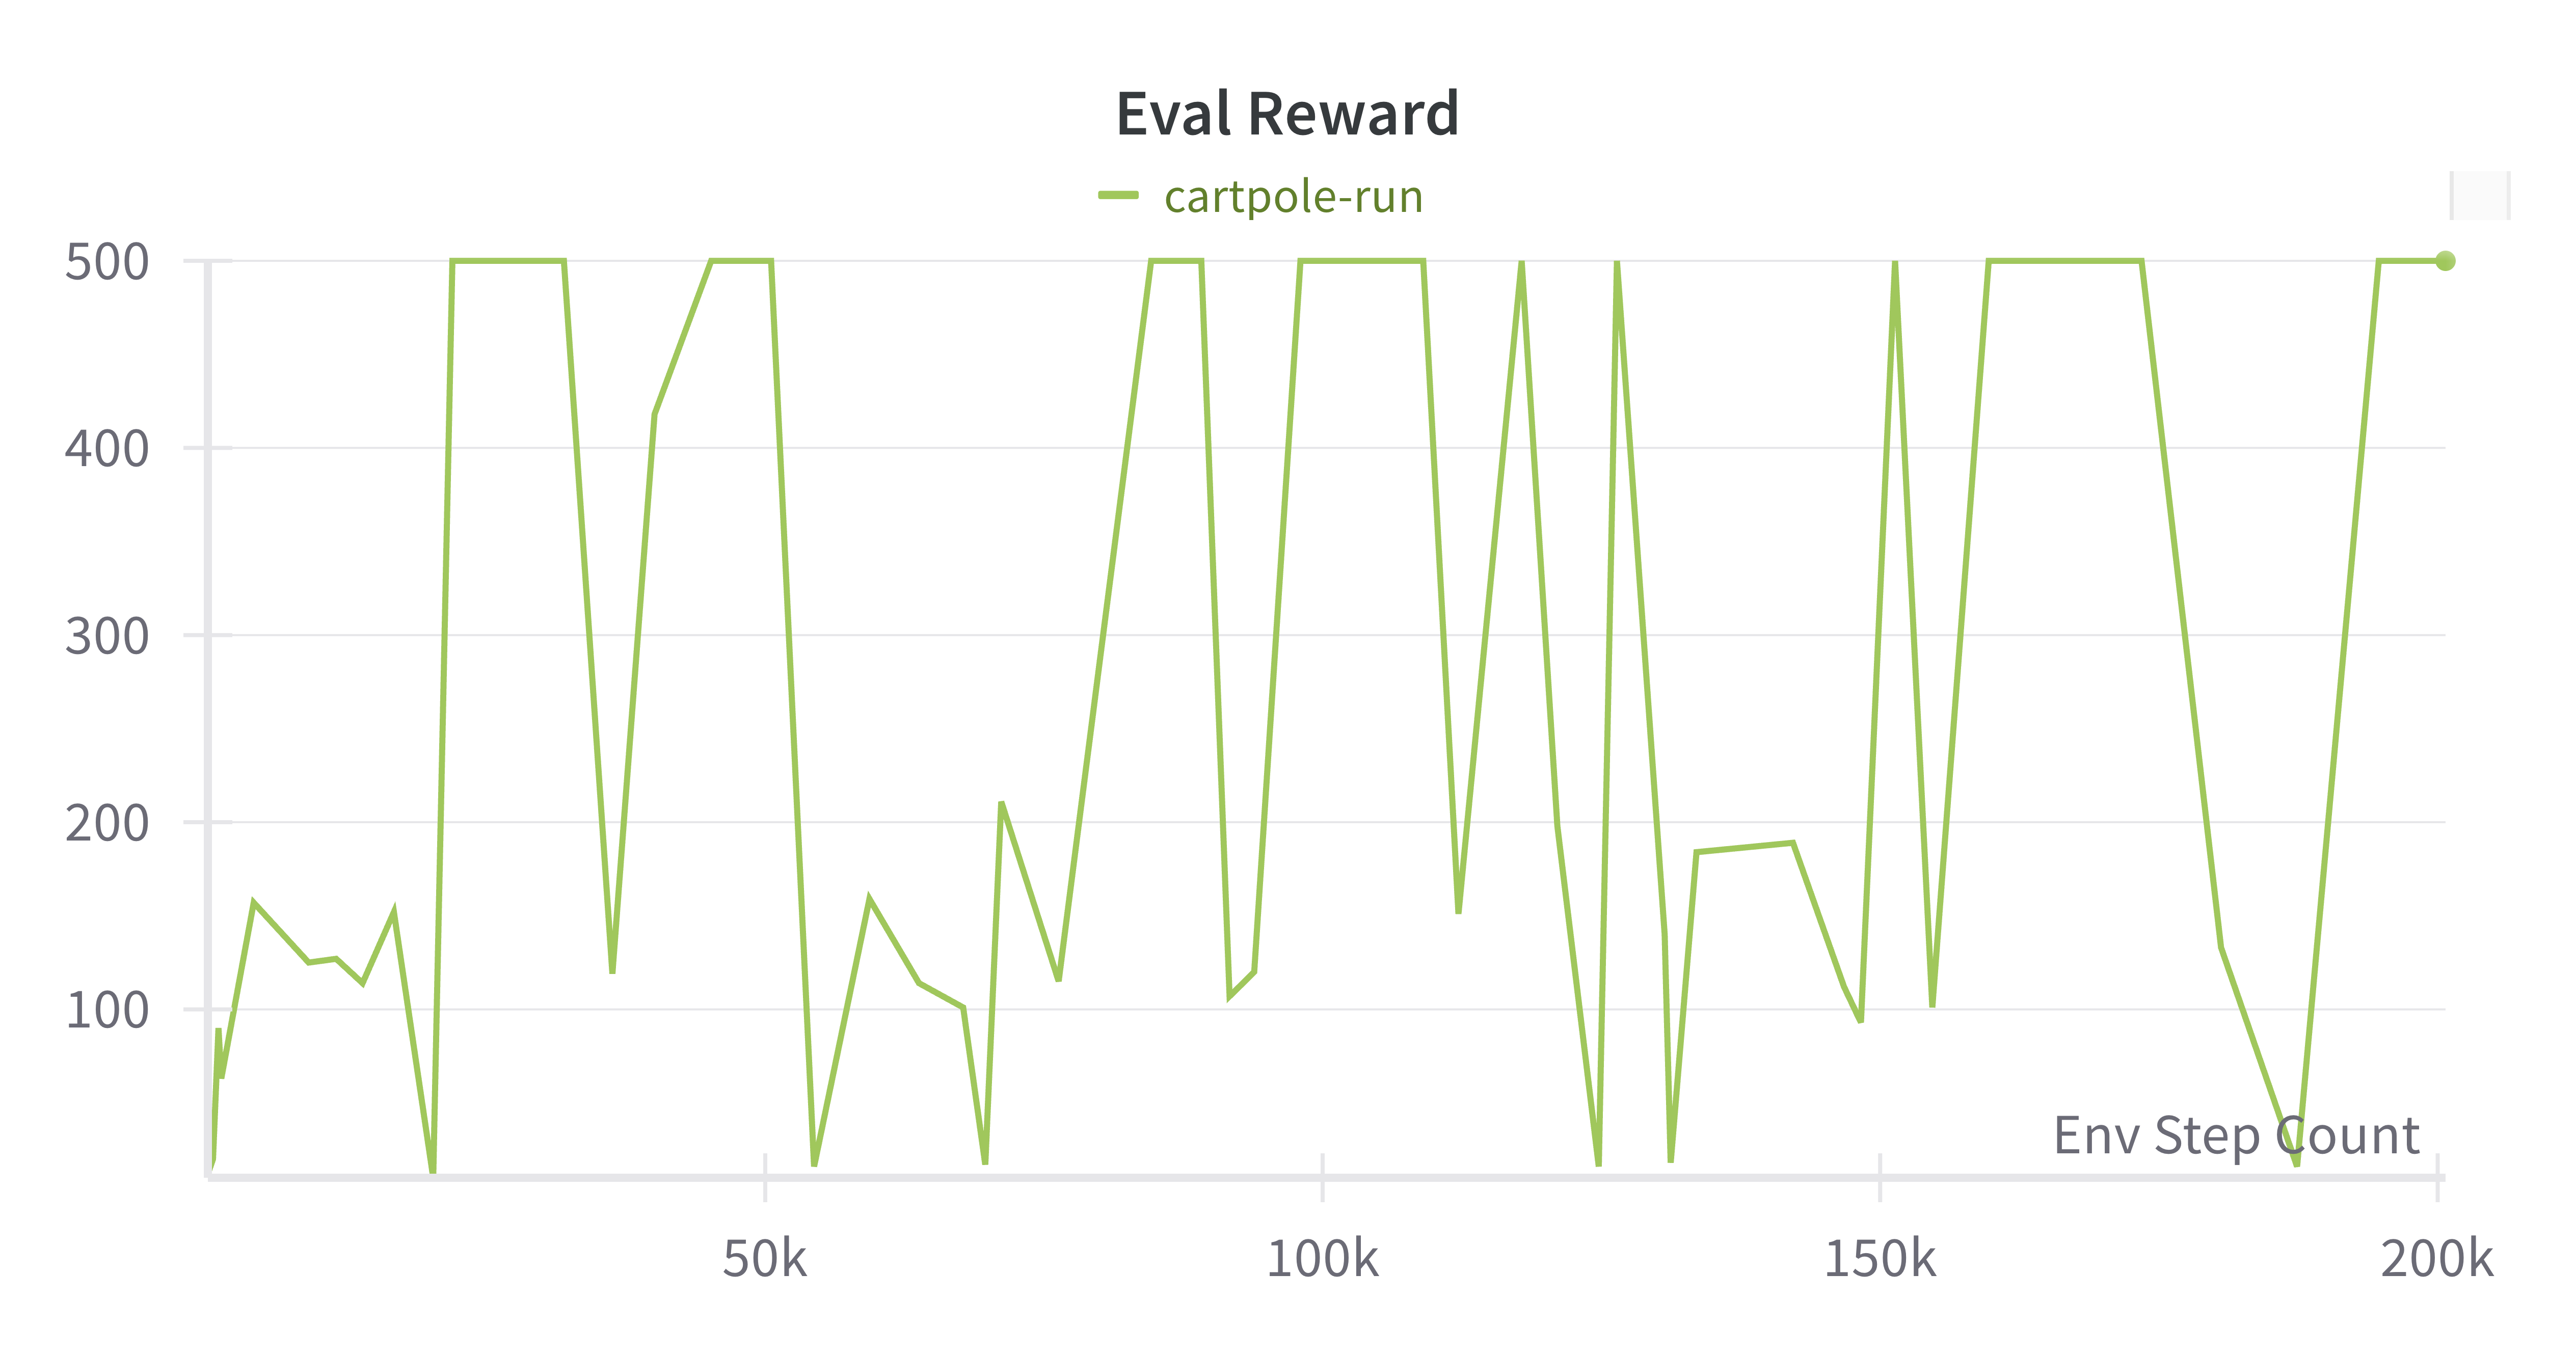
\includegraphics[width=0.5\linewidth]{figures/task1-eval}
\caption{Training curves for CartPole-v1 environment. The x-axis represents environment steps, and the y-axis represents the average evaluation reward.}
\label{fig:task1-eval}
\end{figure}
\begin{figure}[H]
\centering
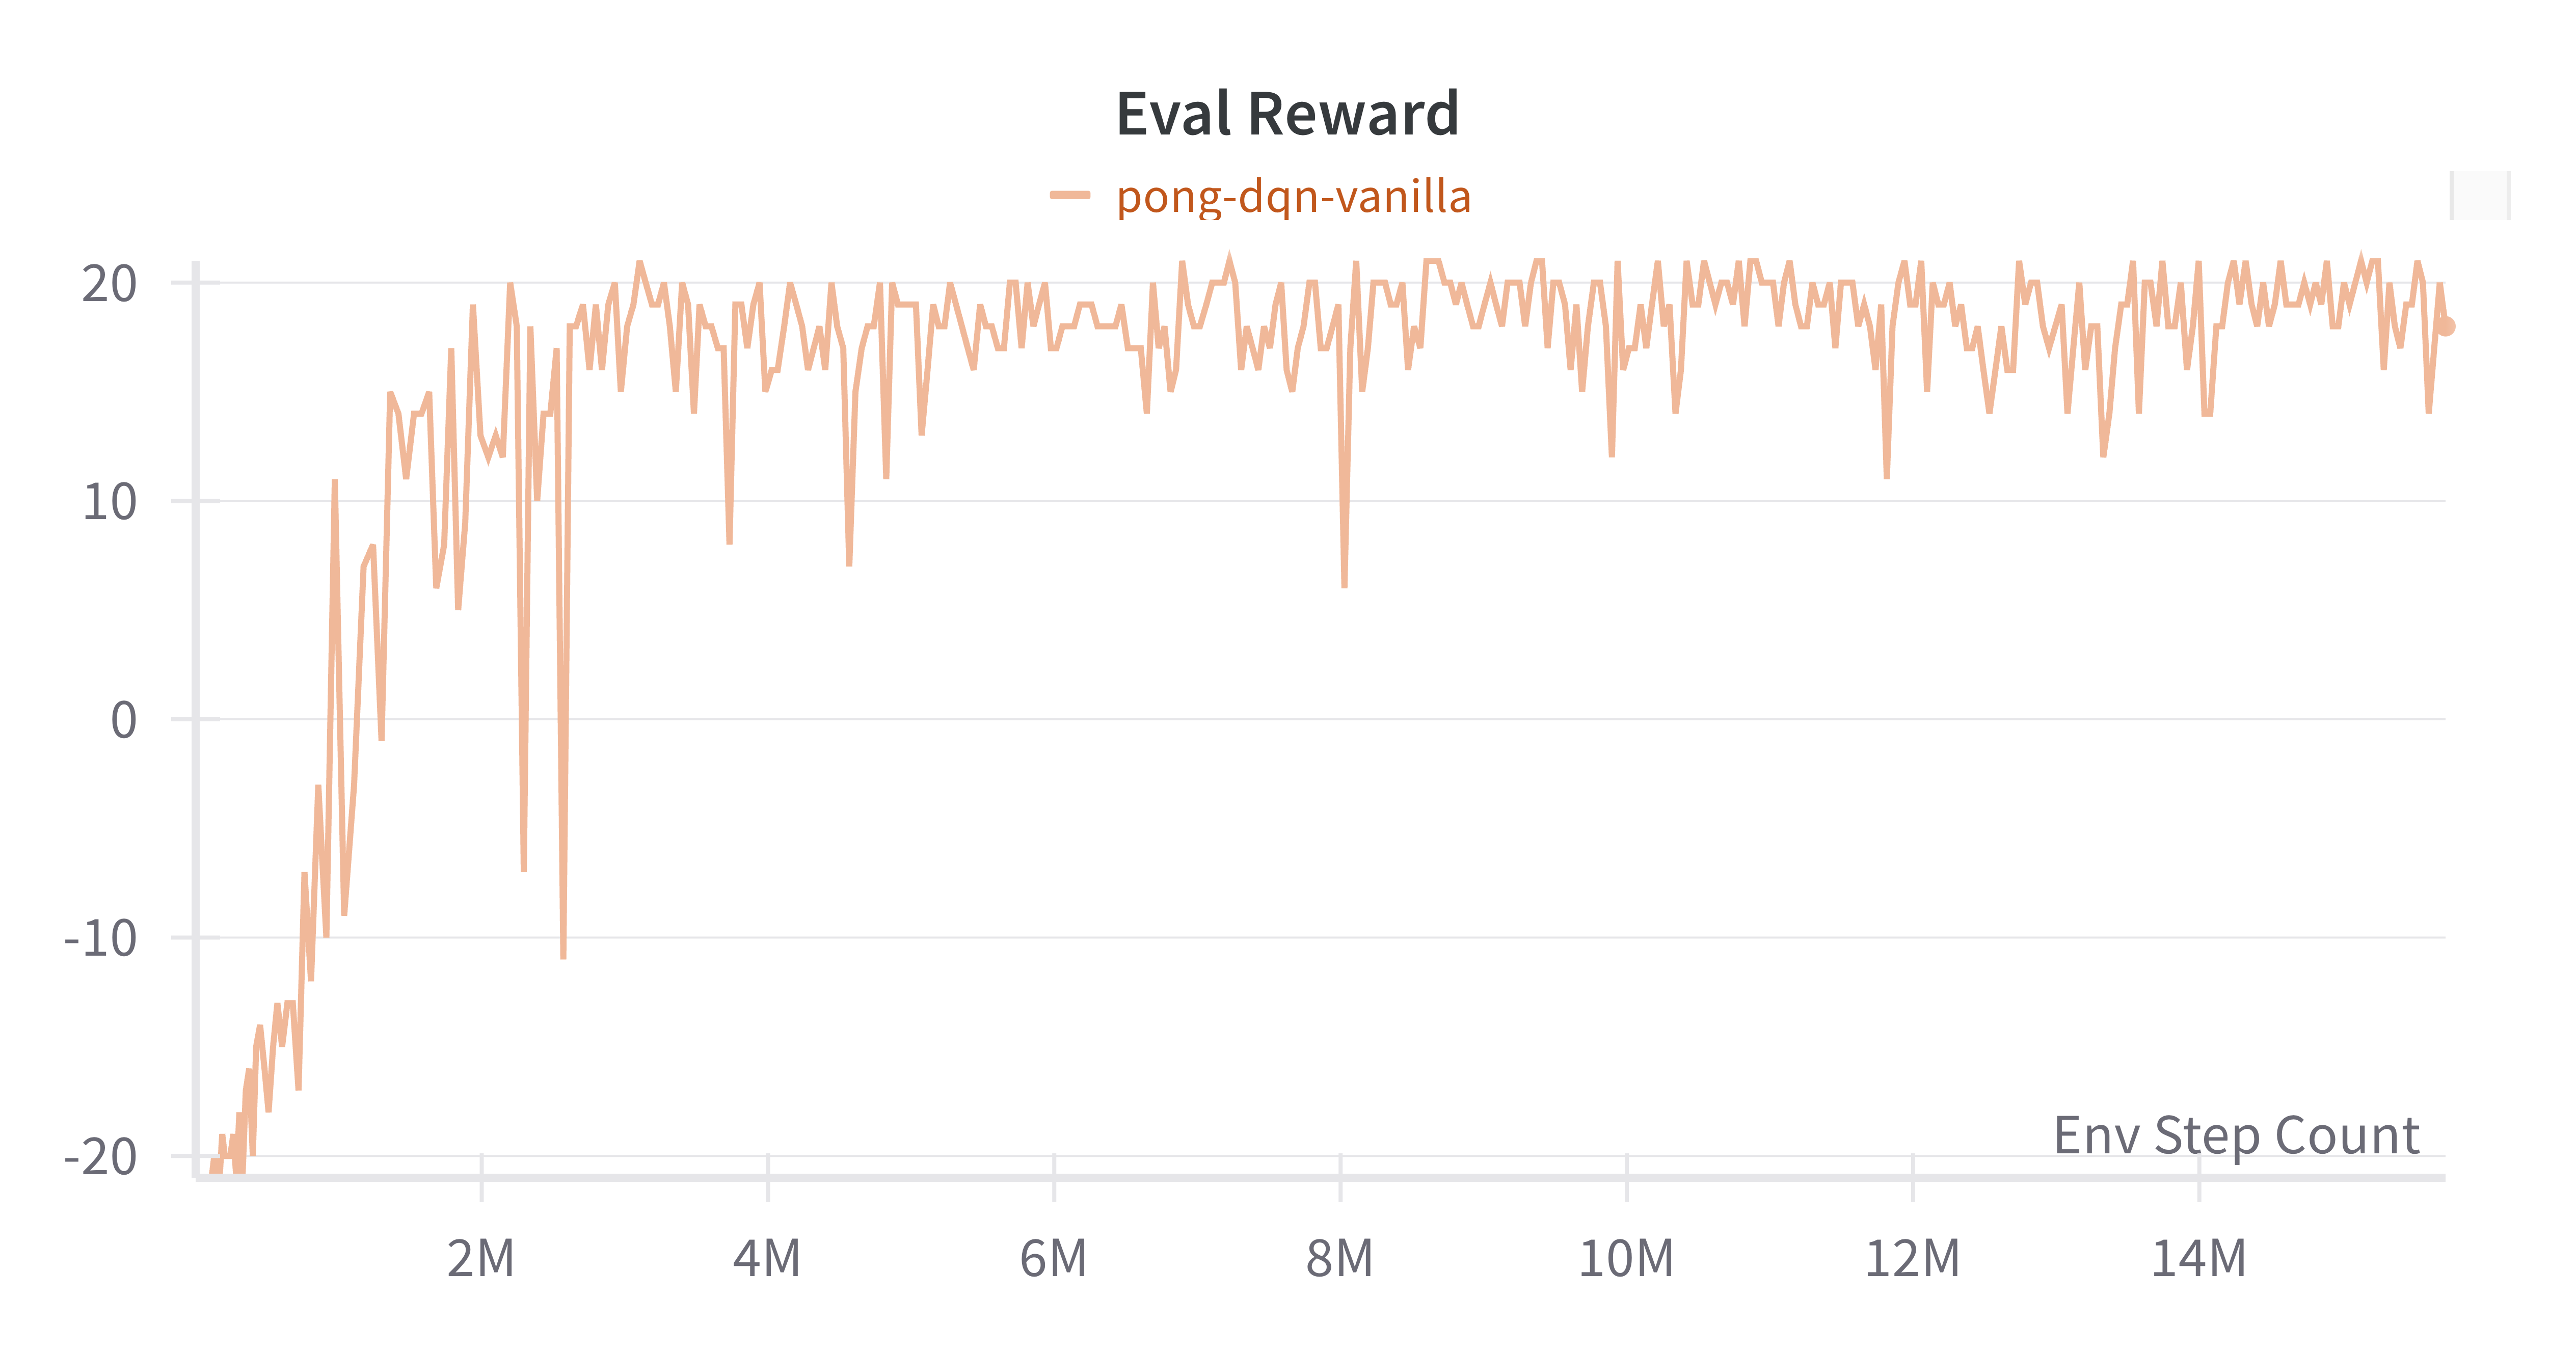
\includegraphics[width=0.5\linewidth]{figures/task2-eval}
\caption{Training curves of vanilla DQN for Pong-v5 environment. The x-axis represents environment steps, and the y-axis represents the average evaluation reward.}
\label{fig:task2-eval}
\end{figure}
\begin{figure}[H]
\centering
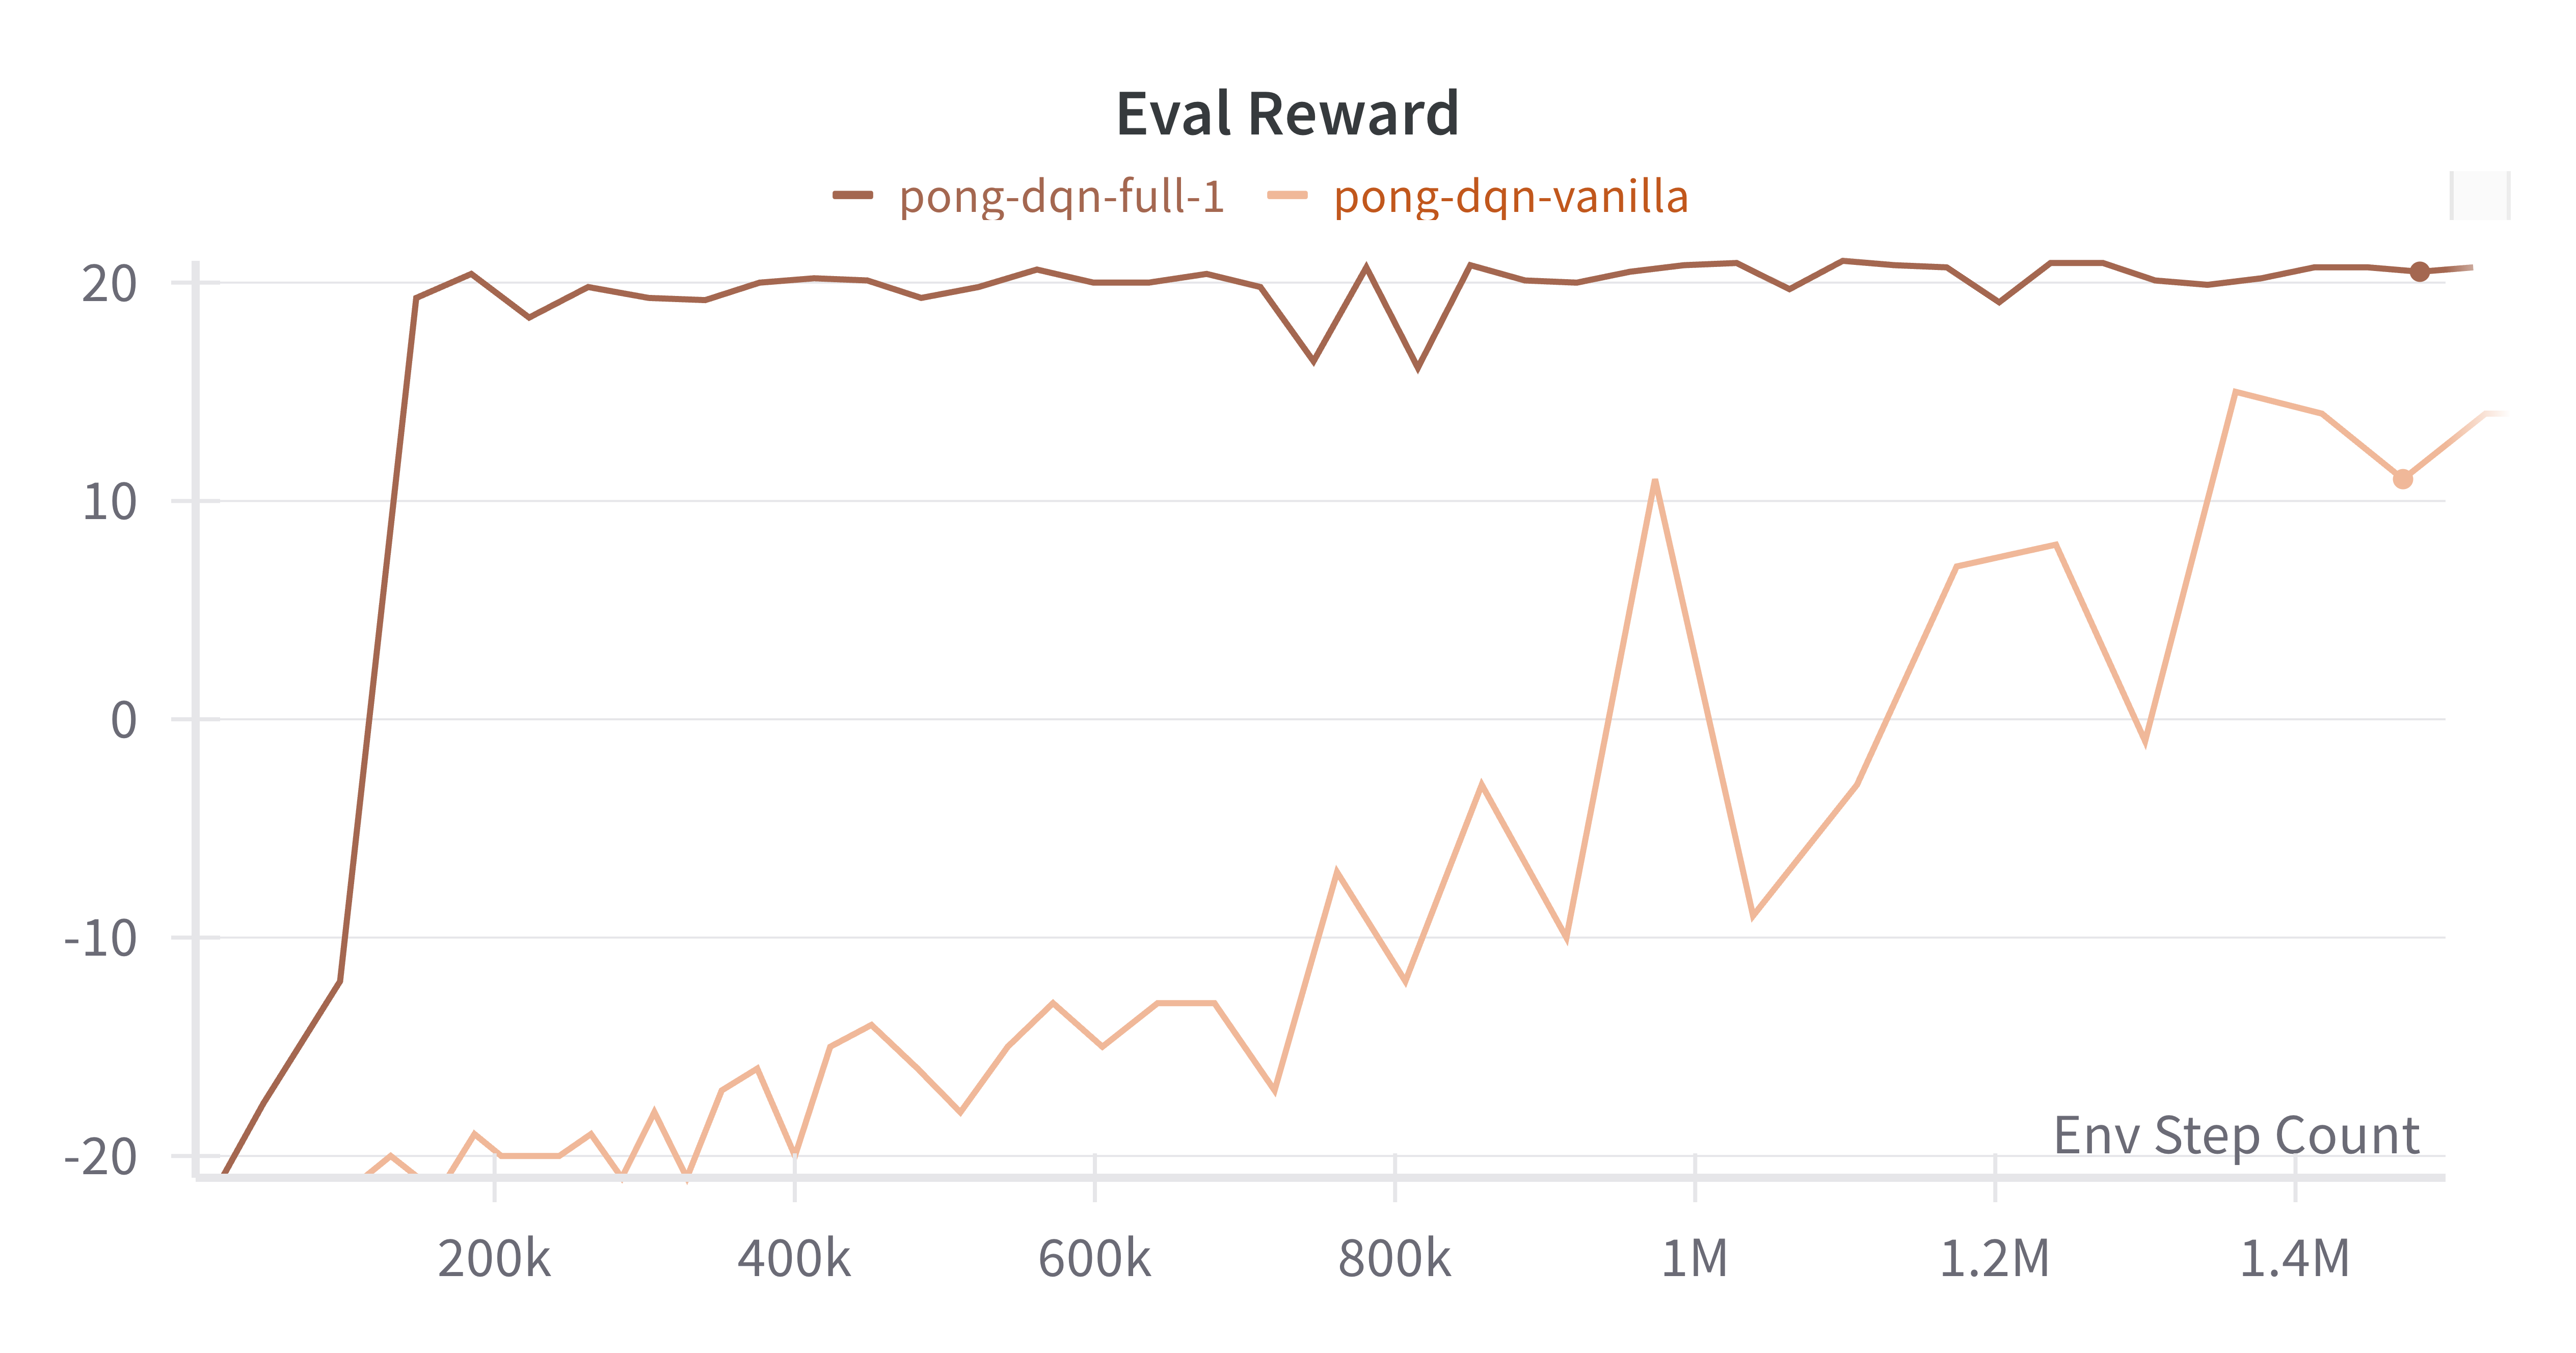
\includegraphics[width=0.5\linewidth]{figures/task3-eval}
\caption{Training curves comparing vanilla DQN and enhanced DQN variants on Pong-v5. The enhanced DQN reaches high performance much faster.}
\label{fig:task3-eval}
\end{figure}

%\begin{figure}[h]
%    \centering
%    \includegraphics[width=0.8\textwidth]{figures/cartpole_training_curve.png}
%    \caption{Training curves for CartPole-v1 environment. The x-axis represents environment steps, and the y-axis represents the average evaluation reward.}
%    \label{fig:cartpole}
%\end{figure}
%
%\begin{figure}[h]
%    \centering
%    \includegraphics[width=0.8\textwidth]{figures/pong_training_curve.png}
%    \caption{Training curves for Pong-v5 environment. The x-axis represents environment steps, and the y-axis represents the average evaluation reward.}
%    \label{fig:pong}
%\end{figure}
%
%\begin{figure}[h]
%    \centering
%    \includegraphics[width=0.8\textwidth]{figures/enhanced_dqn_curve.png}
%    \caption{Training curves comparing vanilla DQN and enhanced DQN variants on Pong-v5. The enhanced DQN reaches high performance much faster.}
%    \label{fig:enhanced}
%\end{figure}

\subsection{Sample Efficiency Analysis}

The enhanced DQN variants demonstrated dramatically improved sample efficiency compared to vanilla DQN. Table \ref{tab:sample_efficiency} presents a comprehensive comparison of environment steps required to reach key performance thresholds across different algorithmic configurations.

\begin{table}[h]
\centering
\caption{Environment steps required to reach specific performance thresholds on Pong-v5. The full enhanced DQN integrates all improvements, while each row below shows the impact of removing a single enhancement from the full configuration.}
\begin{tabular}{lccc}
\toprule
\textbf{Method} & \textbf{Steps to Score 0} & \textbf{Steps to Score 10} & \textbf{Steps to Score 20} \\
\midrule
Vanilla DQN & 969,785 & 1,084,977 & 1,795,184 \\
\midrule
Full Enhanced DQN & \textbf{115,518} & \textbf{115,518} & \textbf{122,834} \\
\midrule
w/o Huber Loss & 156,116 & 191,845 & 471,005 \\
w/o PER & 241,635 & 418,820 & 599,478 \\
w/o Multi-step & 203,658 & 413,582 & $>$750,000 \\
w/o Dueling Network & 144,277 & 180,154 & 249,009 \\
w/o Noisy Network & 126,703 & 189,507 & 451,812 \\
w/o Enhanced Frame Preprocessing & 186,692 & 208,074 & 422,831 \\
\bottomrule
\end{tabular}
\label{tab:sample_efficiency}
\end{table}

The fully enhanced DQN achieves a perfect score of 20 in just 122,834 environment steps, representing a remarkable 14.6× improvement in sample efficiency over the vanilla implementation, which requires approximately 1.8 million steps to reach the same performance. Notably, the enhanced agent reaches an average score of 10 at essentially the same step count as when it reaches a score of 0, indicating extremely rapid learning once it discovers an effective strategy.

\subsection{Ablation Study}

To quantify the contribution of each enhancement, I conducted a comprehensive ablation study by systematically removing one component at a time from the full enhanced DQN configuration. Figures \ref{fig:ablation-eval} and \ref{fig:ablation-total} visualize the comparative learning curves, while Table \ref{tab:sample_efficiency} provides precise step counts for reaching specific performance thresholds.

\begin{figure}[H]
\centering
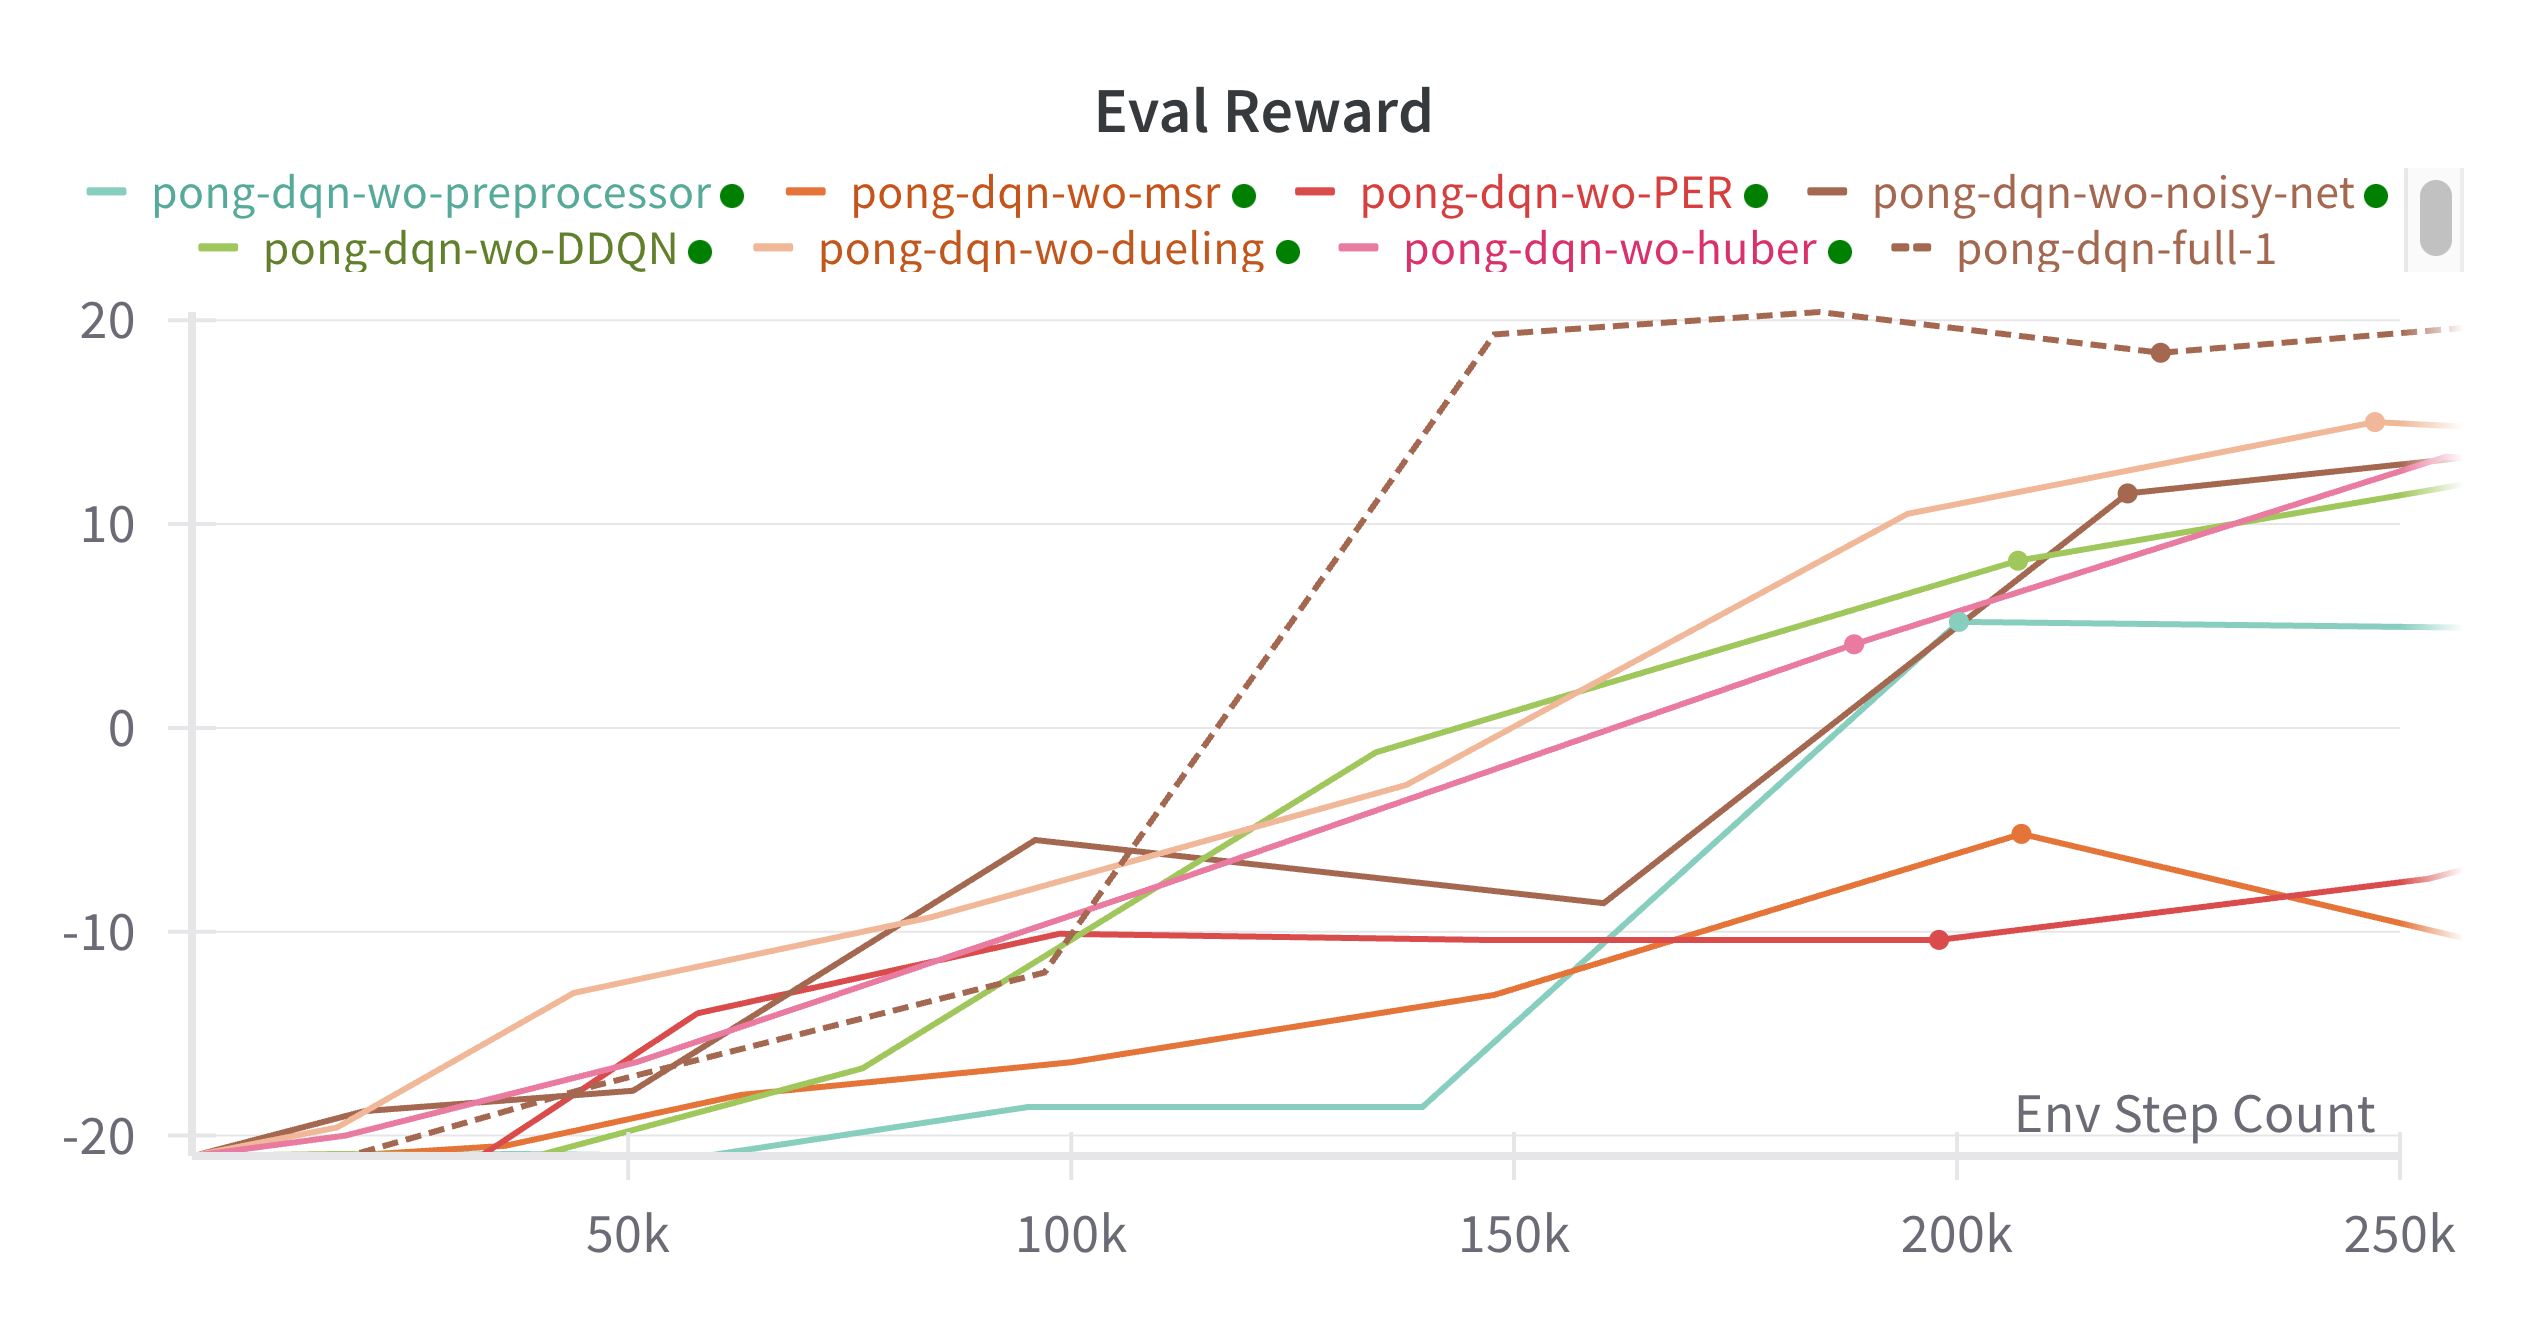
\includegraphics[width=0.5\linewidth]{figures/ablation-eval}
\caption{Evaluation reward curves comparing the full enhanced DQN against variants with single components removed. The steep curve of the full enhanced version demonstrates the synergistic effect of combining all enhancements.}
\label{fig:ablation-eval}
\end{figure}

\begin{figure}[H]
\centering
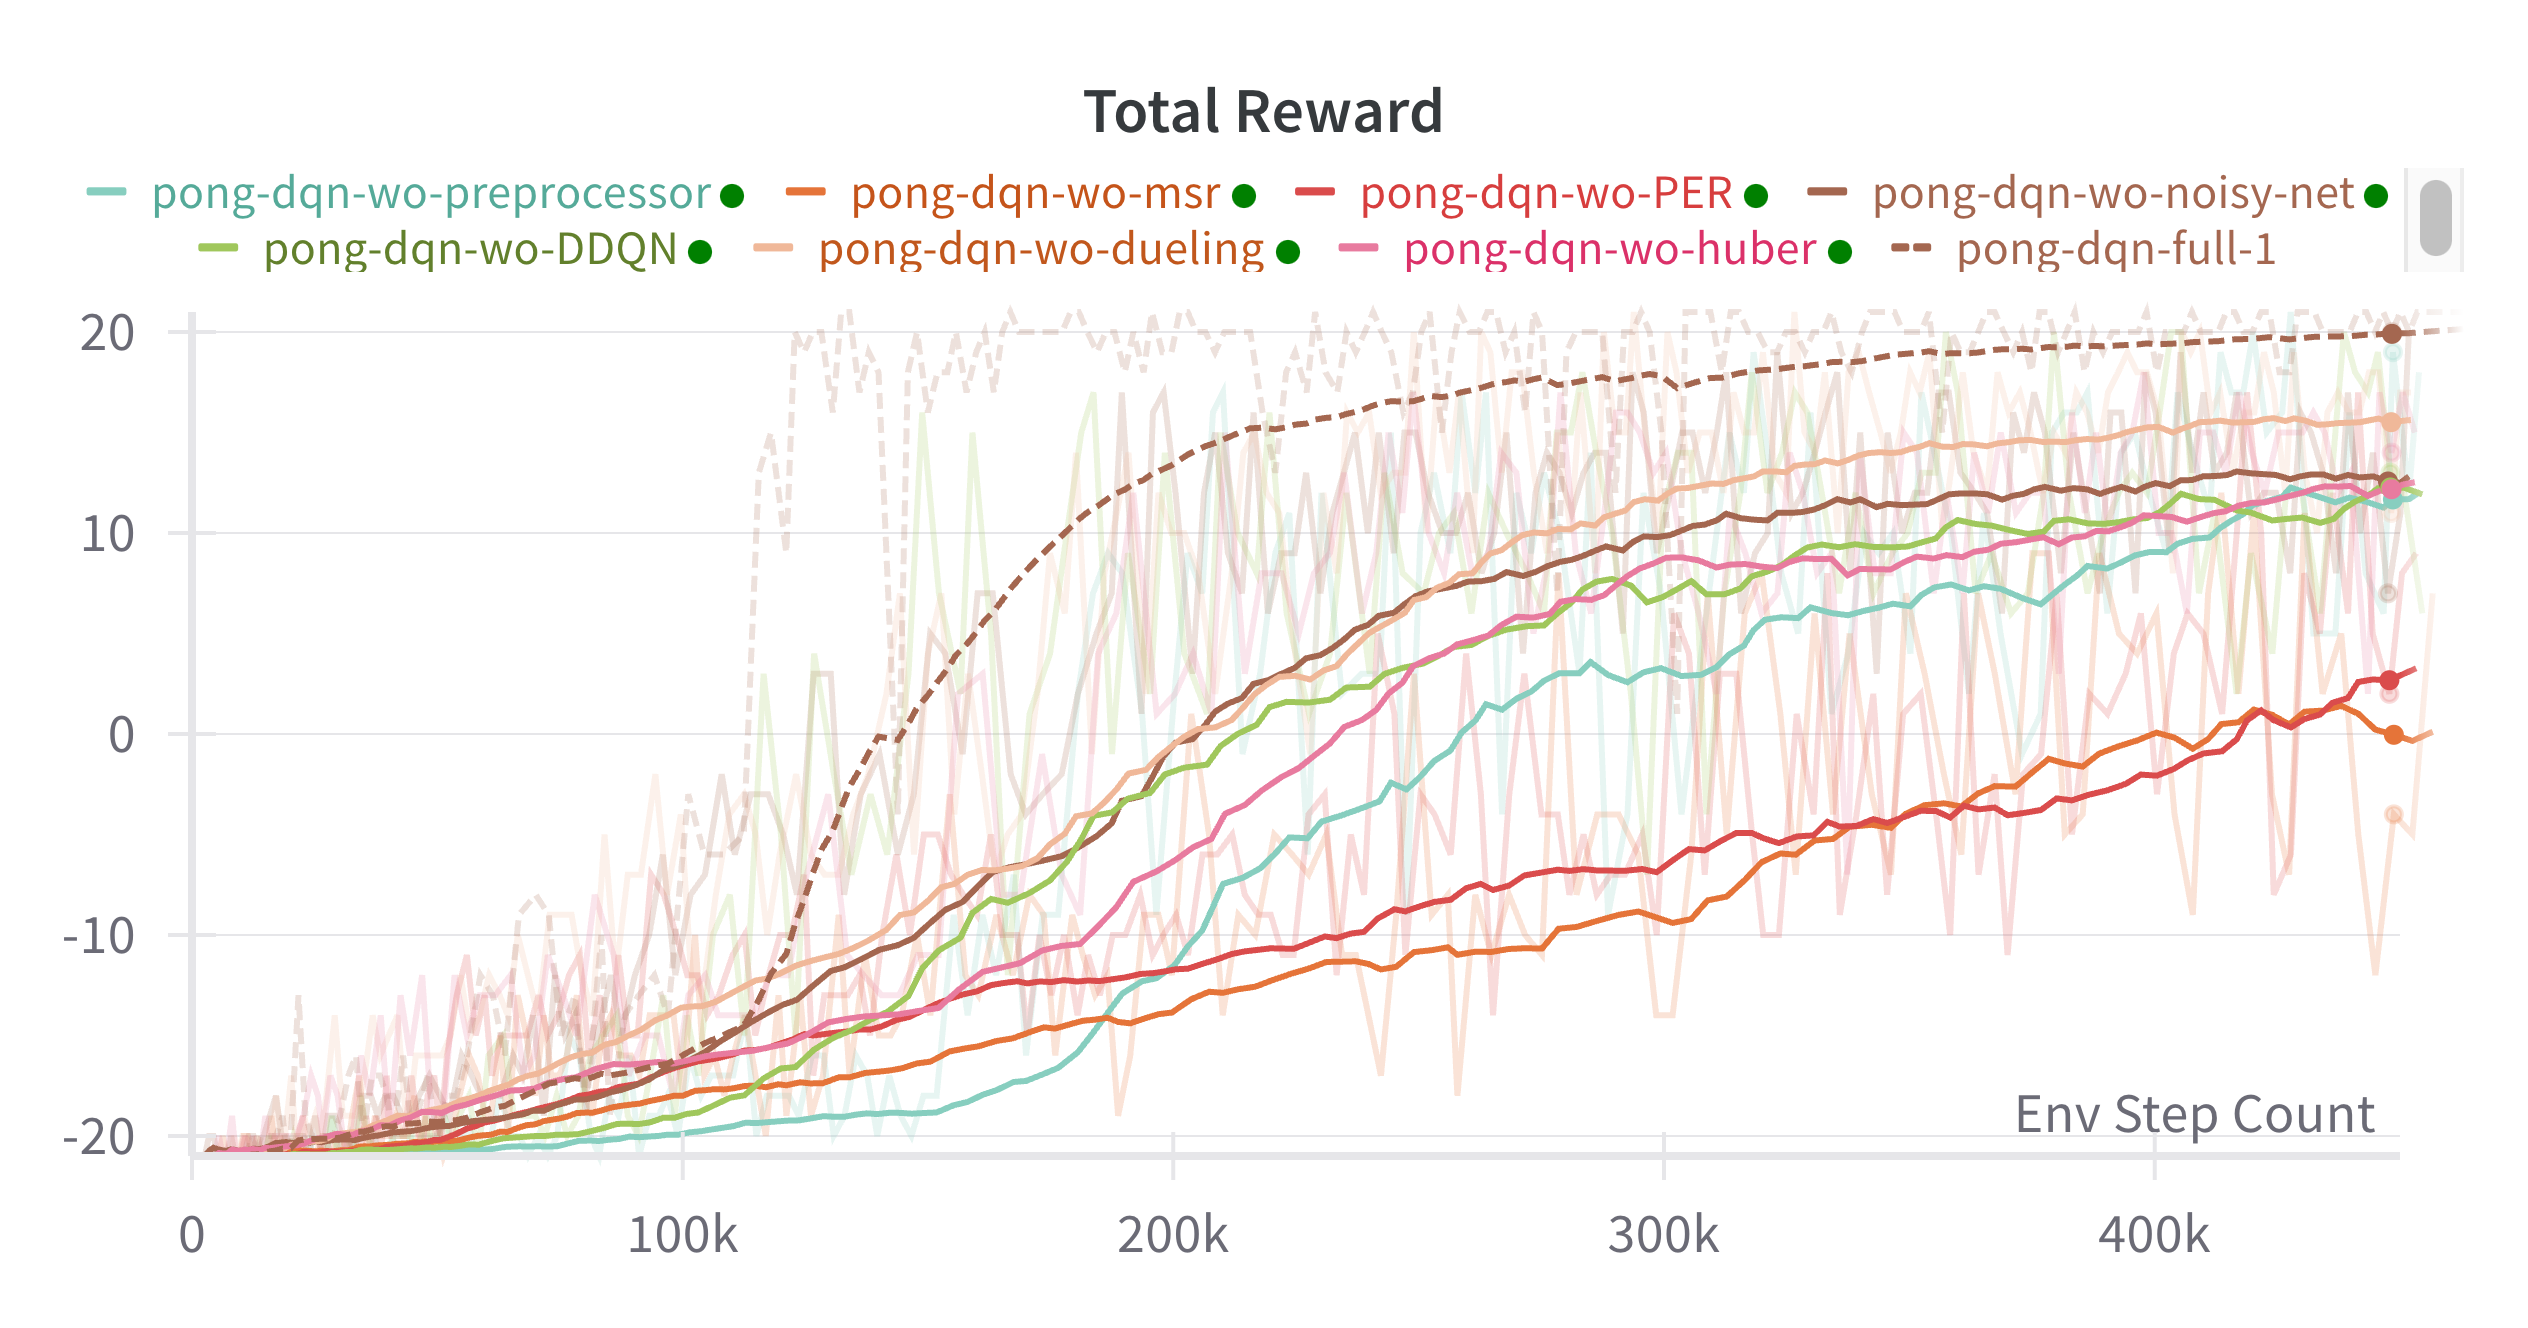
\includegraphics[width=0.5\linewidth]{figures/ablation-total}
\caption{Total reward across training for different DQN variants. This metric captures both the learning speed and stability of each configuration, with higher area under the curve indicating more efficient learning.}
\label{fig:ablation-total}
\end{figure}

The ablation results reveal specific contributions from each component:

\begin{itemize}
    \item \textbf{Prioritized Experience Replay (PER):} Produced the most significant individual impact. The annealing of the $\beta$ parameter from 0.4 to 1.0 was crucial for balancing initial learning speed with long-term stability by gradually correcting the sampling bias.
    
    \item \textbf{Multi-step Return:} The second most impactful enhancement. Using $n=3$ provided an optimal balance between bias reduction and variance control. This approach was particularly valuable in Pong due to the delayed nature of rewards.
    
    \item \textbf{Huber Loss:} While having modest impact on early learning. This suggests its outlier resistance becomes increasingly important in later stages of policy refinement when the agent is making smaller, more precise adjustments.
    
    \item \textbf{Noisy Networks:} This technique proved particularly effective in Pong, where strategic exploration around promising ball trajectories is more valuable than random paddle movements provided by $\epsilon$-greedy exploration.
    
    \item \textbf{Enhanced Frame Preprocessing:} Binary thresholding and proper cropping contributed substantially to efficiency. These enhancements enabled the convolutional layers to more quickly identify key game elements.
    
    \item \textbf{Dueling Network:} While showing the smallest individual impact, the dueling architecture provided consistent benefits across all training stages. Its separation of state value and action advantage estimation proved particularly effective in Pong, where understanding good positions (state value) can be learned somewhat independently from optimal paddle movements (action advantage).
\end{itemize}

The most striking finding from this ablation study is that the combined effect of all enhancements far exceeds what would be expected from their individual contributions. This synergistic interaction occurs because each enhancement addresses a different limitation of the base DQN algorithm:

\begin{enumerate}
    \item PER focuses computation on valuable experiences
    \item Multi-step returns address the delayed reward problem
    \item Huber loss improves optimization stability
    \item Noisy networks provide adaptive exploration
    \item Enhanced preprocessing simplifies the feature learning challenge
    \item Dueling architecture decouples state value and action advantage learning
\end{enumerate}

When combined, these enhancements create a virtuous cycle where improvements in one aspect amplify the benefits of others. For example, better exploration from noisy networks discovers more informative experiences, which PER then prioritizes for learning, while multi-step returns help propagate the resulting value information more effectively through time. This mutually reinforcing system explains why the full enhanced DQN achieves such dramatic performance improvements over vanilla DQN.

\section{Additional Analysis}

\subsection{Training Instability in DQN}

\begin{figure}[H]
\centering
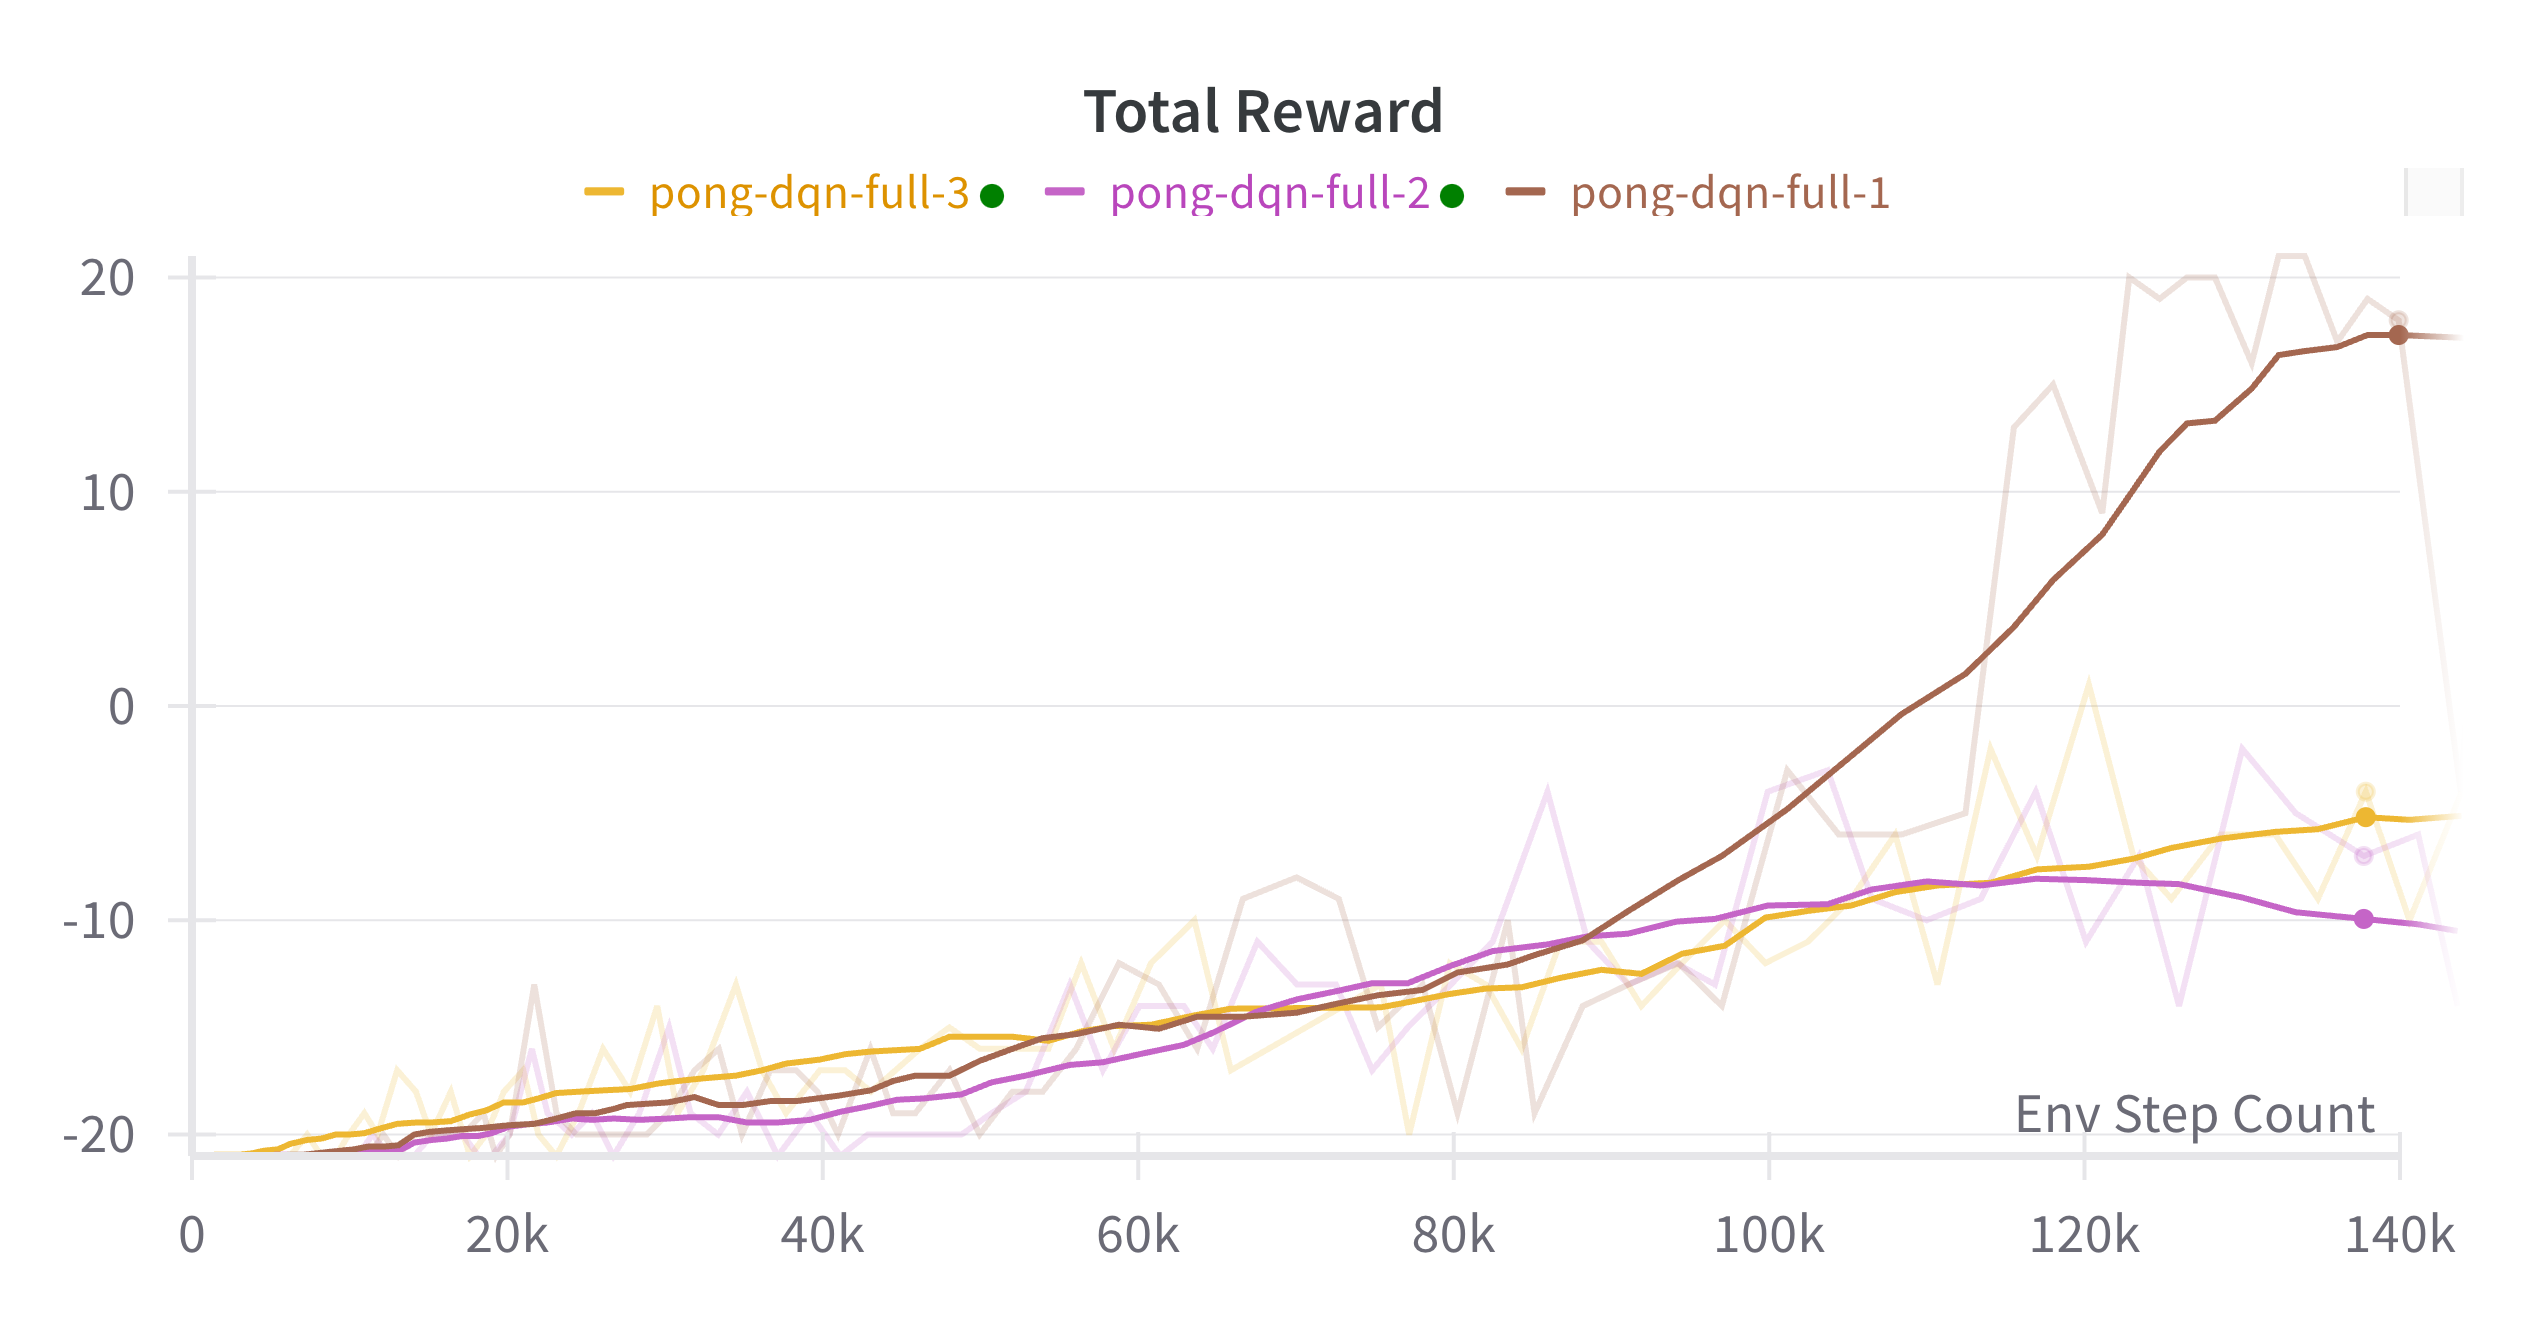
\includegraphics[width=0.5\linewidth]{figures/unstable}
\caption{The instability issue in the DQN training process.}
\label{fig:unstable}
\end{figure}


Throughout the training process, I observed that DQN exhibits significant training instability even when using identical hyperparameter configurations. As shown in Figure \ref{fig:unstable}, three training runs with the same hyperparameters can yield remarkably different learning curves and final performance.

This instability can be attributed to several factors:

\begin{enumerate}
    \item \textbf{Initialization sensitivity}: Small differences in network weight initialization can be amplified through the bootstrapping process in Q-learning, where current value estimates depend on previous estimates.
    
    \item \textbf{Experience replay sampling variance}: The stochastic nature of experience replay sampling introduces variability between runs. Even with prioritized replay, the subset of experiences used for each update can significantly impact gradient direction and magnitude.
    
    \item \textbf{Environment stochasticity}: In environments with inherent randomness (like starting positions in Pong), different trajectories can lead to entirely different learned strategies.
    
    \item \textbf{Non-stationarity}: The Q-learning target is non-stationary, as it depends on the current network's estimates, creating a "moving target" problem that can lead to oscillations during training.
\end{enumerate}


This observation highlights the importance of running multiple seeds when evaluating DQN variants and suggests that single-run comparisons between algorithms may lead to misleading conclusions.

Nonetheless, I think the ablation studies still show the effectiveness of each components.

\subsection{Emergent Exploitative Strategy in Pong}

I analyze the best-performing model, which achieved an average score of 19 within just 140K environment steps, revealed an interesting phenomenon. The agent discovered an exploitative strategy that was remarkably effective against the built-in AI opponent.

The agent learned to position its paddle at a specific vertical position where the opponent's algorithm consistently failed to return the ball. This position appears to exploit a blind spot in the opponent's control algorithm, causing it to misjudge the trajectory of the ball and miss consistently.


\section{Conclusion}

In this lab, I successfully implemented and enhanced the Deep Q-Network algorithm for reinforcement learning in both CartPole and Pong environments. The vanilla DQN implementation achieved strong performance in both tasks, while the enhanced DQN demonstrated dramatically improved sample efficiency, particularly in the more complex Pong environment.

The ablation study revealed that while each enhancement contributed to performance improvements, the combination of all techniques yielded synergistic benefits that exceeded the sum of individual contributions. This highlights the importance of a holistic approach to algorithm design in deep reinforcement learning.

Future work could explore additional enhancements such as distributional RL approaches (C51, QR-DQN) and curiosity-driven exploration. Integration with more complex environments like 3D games would also be an interesting extension of this work.


\printbibliography
\end{document}